% !TEX encoding = UTF-8 Unicode
% !TEX TS-program = pdflatex
% !TEX spellcheck = en-US
% !TEX root = ../Report.tex

\chapter{Version Control System}
As suggested by the definition, a version control system (VCS) is a system responsible for the management of changes to documents. One of the most important advantages of using a version control system during a design process involving software programs is to strongly facilitate the team work. Since we worked on this project as a group, we decided to fully take advantage of a supporting system, such as Git. n particular, it allowed us to keep trace of each single change each team member was implementing. As a matter of fats, it allowed us to revert a specific document to a previous revision, enabling each team member to track each other's edit and correct possible mistakes. The other key features, provided by Git, which really helped us was the possibility to \textit{merge} together our own WCs (working copies). In this way, each time more than one team members were committing some changes about the same file, we could merge both the new revisions, without loosing anything. 

Inside the current chapter, we are going to show how we have configured the Git version control system itself and with all the other software programs we used.
\section{Setup Git control on Matlab}
Inside this section we are going to report how we implemented the Git operating conditions and their requirements into Matlab. This step was the most critical one because the Matlab software is not completely pre-designed to work under the Git management. In order to setup the correct operating conditions, we set some initial configurations. To avoid following troubles, we followed, step by step, the documentation about "setup Git control" directly provided by Matlab.

Since there are a lot of different ways to use Git, we decided to adopt the original one, the command-line tool, because it is the only one able to run all the Git commands. In order to take advantage of all the Git features, the first step was about verifying if there was installed a command-line Git client and if it was available at system level. 

The second important configuration we set was related to both Matlab and Simulink file extensions (.mlx, .mat, .fig, .slx) format. As a matter of facts, by following the Matlab documentation about "setup Git control", we learned that, Git, manages binary format files. Matlab, instead, does not. If we had worked without register the "new" file extension, we would have got problems such as corrupting our files when we were submitting them by substituting keywords, or attempting to automerge, for example. We solved that problem by inserting conflict markers. To make it real, we modified the .gitattributes file to register binary files, as the fig. \ref{gitattributes} will show. 
\begin{figure}
	\centering
	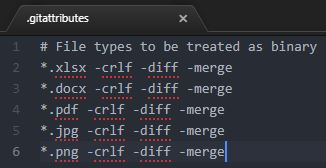
\includegraphics[scale=1]{../Images/VCS/Gitattributes.JPG}
	\caption{Git Setup file - .gitattributes}
	\label{gitattributes}
\end{figure}
These lines simply specify that Git will not try automatic line feed, diff, and merge attempts for these types of files. Moreover, it is possible to see even the figure file formats, .jpg and .png, due to our need of showing our final results.

The next step was related to the .gitignore file. Actually, in general, not each file created or updated should be committed inside the repository. For example, temporary files from the development environment, test outputs, and logs are file types that are always created but these are not part of the codebase. Git provides a specific tool, the .gitignore file, used to specify all these previous file types we want to neglect.

In order to activate this feature, we have modified our .gitignore file including specific files types inside our repository. In such a way, each time a team member was committing some changes, Git started ignoring them. Finally, to make it available for each team member instead of just for the local system which was modifying it, we have commited these changes inside our repository. The .gitignore file we pushed is clearly visible inside fig. \ref{gitignore}.
\begin{figure}
	\centering
	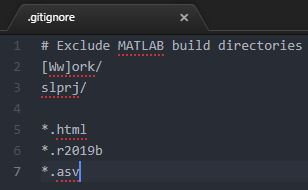
\includegraphics[scale=1]{../Images/VCS/Gitignore.JPG}
	\caption{Git Setup file - .gitignore}
	\label{gitignore}
\end{figure}
\section{Git repository architecture}
As we previously said at the beginning of current chapter, the main purpose of a version control system is to manage all the occurred changes to a specific set of data, over time. This set of data can be structured in different ways. In order to better understand how we organized our repository, in terms of main trunk, branches and so on, there follows the fig. \ref{tree1} and \ref{tree2} showing our development line structure, in both Matlab and Git platforms.
\begin{figure}
	\centering
	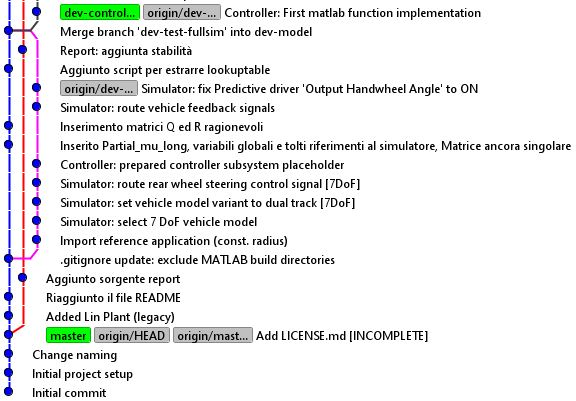
\includegraphics[scale=0.6]{../Images/VCS/VCS_tree.JPG}
	\caption{Virtual Control System - Working Tree (Matlab platform)}
	\label{tree1}
\end{figure}
Before listing all the branches we adopt and the criteria we followed, we want to better clarify both the four-wheels steering project purpose and how we designed it. The final project aim was related to control, by means of an optimal control tool (LQR), the vehicle behaviour in terms of both angular speed ($\omega_{z}$) and side-slip angle ($\beta_{u}$). To do so, we built the vehicle model, then we chose a pre-built vehicle simulator to physically check our changes and finally we designed the controller. To avoid mixing together too many project sub-sections, at the beginning we created 3 main branches, each one starting from the trunk:
\begin{itemize}
	\item dev-model: related to vehicle modeling;
	\item dev controller: related to the controller design;
	\item dev-report: related to drafting of report ;
\end{itemize}
Later on, due to all the design bumps in the road we met during project development, we created other "sub-branches" (as dev-sim-integration, dev-test-fullsim, etc.) starting from both dev-model and dev-controller. This was done in order to deal with each single development topic (of the overall project) inside its own apposite branch. In this way, we could manage every issue without compromising the entire work. After solving all the single troubles, we merged the created sub-branches into the main one, dev-model or dev-controller, specifically. 

Finally, once we completed the job, we merged both dev-controller and dev-report inside dev-model, in order to obtain a final branch containing the overall project development. Then, as the last step, we merged dev-model into the master line, the trunk, creating the first ever release of our project.

In the bottom area of fig.\ref{tree1}, it is possible to see the trunk, we called \textit{master}, highlighted in green fluo.
while in the top one there is the branch called \textit{dev-controller}.
\begin{figure}
	\centering
	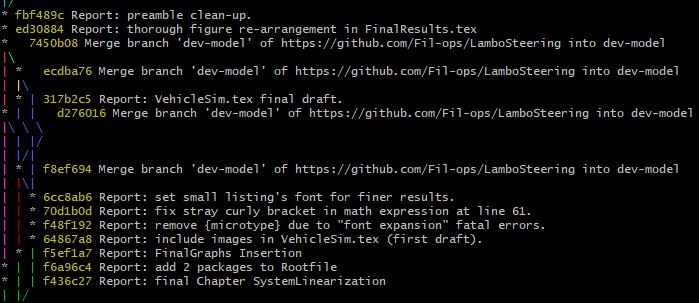
\includegraphics[scale=0.6]{../Images/VCS/VCS_Git_tree.JPG}
	\caption{Virtual Control System - Working Tree (Git platform)}
	\label{tree2}
\end{figure}